%%% Dokumentenklasse und Layout 
\documentclass[fontsize=12pt,a4paper,headinclude=no,headings=small]{scrartcl}

%%% Ränder
%\usepackage{typearea}
\areaset{180mm}{230mm} % Der gewünschte Satzspiegel

%%% Sprache, Rechtschreibung, Silbentrennung
\usepackage[ngerman]{babel} 	% Deutscher Text
\usepackage[T1]{fontenc}			% Trennung von Umlauten enthaltenden Woertern
\usepackage[utf8x]{inputenc} 	% Erlaubt Eingabe von Umlauten (kein "a etc. notwendig). 
\usepackage[right]{eurosym}		% Euro-Symbol verwendbar (durch \euro)

%%% Darstellung, Formatierung
\addtokomafont{sectioning}{\rmfamily} 	% Serifen in Überschrift
\clubpenalty = 1000 			% reduziert Schusterjungen
\widowpenalty = 1000 			% reduziert Hurenkinder
%\usepackage{ae,aecompl}			% schönere Schriftart (Vektorfonts)

%%% Links für pdflatex
\usepackage{hyperref}	% PDF Referenzen klickbar
\usepackage{url}		% URLs klickbar

%%% Tabellen und Grafiken, Listen
\usepackage{graphicx}	% Grafiken einbinden
\usepackage{pdfpages}		% PDFs einbinden
\usepackage{float}
\usepackage{tabularx}
\usepackage{dcolumn}
\usepackage{multicol}
%\setlength{\columnseprule}{1pt}
%\setlength{\columnsep}{10pt}
\newcolumntype{C}{>{\centering\arraybackslash}X}
\newcolumntype{R}{>{\arraybackslash}X}
%\usepackage[skip=0pt,labelfont=it,nooneline,hang,small]{caption}
\usepackage{enumerate}

%%% Listing
\usepackage{listings}
% a listing environment that doesn't allow page breaks
\lstnewenvironment{code}[1][]%
  {\minipage{\linewidth} 
   \lstset{basicstyle=\ttfamily\footnotesize,frame=single,#1}}
  {\endminipage}

%%% Farben (Farben siehe: http://en.wikibooks.org/wiki/LaTeX/Colors)
\usepackage{color}

%%% TikZ
\usepackage{pgf}
\usepackage{tikz}
\usetikzlibrary{arrows,automata}

%%% Mathe
\usepackage[fleqn]{amsmath}
\usepackage{amssymb}
\usepackage{amsthm} % Umgebung für Beweise und Theoreme
%\usepackage{amsfonts}
\allowdisplaybreaks % Alignment Umgebung darf auf mehrere Seiten umbrechen
\usepackage{dsfont}

%%% Header
\usepackage{fancyhdr}
\pagestyle{fancy}
\setlength{\headheight}{30pt}
\lhead{Hausaufgabe zur Vorlesung \\\emph{Mobile und verteilte Datenbanken}}
\rhead{Dennis Krüger ()\\Martin Thurau (612016)}
\renewcommand{\headrulewidth}{0.4pt}
\renewcommand{\footrulewidth}{0.4pt}
\chead{}

%%% eigene Befehle
\newcommand{\footurl}[1]{\footnote{\url{#1}}}
% TODO und FIXME
  \newcommand{\todo}[1]{\colorbox{yellow}{\textbf{TODO} #1}}
  \newcommand{\fixme}[1]{\colorbox{red}{\textbf{FIXME} #1}}
% Sequenz
  \newcommand{\seq}[1]{\ensuremath{\left \langle #1 \right \rangle }}
% Mengen (mit und ohne "`für die gilt"' Bedingung
  \newcommand{\set}[1]{\ensuremath{\left\lbrace {#1} \right\rbrace }}
  \newcommand{\condset}[2]{\ensuremath{\left\lbrace #1 \;\middle|\; #2 \right\rbrace }}

%%% Mathe Operatorentype filter text
\renewcommand{\div}{\ensuremath{\text{ div }}}
\renewcommand{\mod}{\ensuremath{\text{ mod }}}
\DeclareMathOperator{\ef}{emptyfile}
\DeclareMathOperator{\es}{empty}

\begin{document}

\section{Verteiltes Sortieren}
\subsection{Umgebung}\label{sort:umgebung}
Um das verteilte Sortieren sinnvoll Testen zu können, ist es notwendig die Ausführung auf mehrere Rechner zu verteilen. Eine rein lokale Ausführung würde zum einen keinen realistischen Kommunikationsoverhead bedeuten und zum anderen wäre die Ausführung an die Leistungsfähigkeit der lokalen CPU gebunden.

Die Messreihen wurden daher auf virtuellen Maschinen in der Amazon Elastic Compute Cloud (Amazon EC2)\footurl{http://aws.amazon.com/ec2/} ausgeführt. Die Ausführung erfolgte dabei jeweils für Server und jeden Client getrennt auf einer eigenen "`Micro"'-Instanz. Die Durchführung der Testreihen wurde mit Hilfe von Python, Fabric\footurl{http://fabfile.org} und boto\footurl{http://code.google.com/p/boto/} automatisiert und ausgeführt.

\subsection{Durchführung der Messung}\label{sort:messung}
Die Performance-Messung wird ausschließlich auf dem Server durchgeführt. Der Server misst dabei, wie viele Millisekunden er für das Einlesen der zu sortierenden Daten, zum verteilen der Daten an die Clients, sowie zum Iterieren über die sortierten Ergebnisse benötigt. Außerdem wird noch die gesamte Ausführungszeit gemessen. Da es sich bei der Umgebung, in der das Sortieren durchgeführt wird, um virtuelle Maschinen handelt, ist die Ausführungszeit natürlich abhängig von der Auslastung der physikalischen Hosts. Es ist jedoch davon auszugehen, dass aufgrund der Tatsache, das Amazon die Instanzen über viele Rechner verteilt, ein brauchbarer Mittelwert entsteht.

\subsection{Parameter der Messungen}
Die Messreihen wurden jeweils mit 2, 4, 8 und 16 Sortierclients und einem Server durchgeführt. Dabei wurden jeweils die Blockgrößen 10, 100, 1000 und 10000 getestet. Für die lokale Sortierung gelten diese Parameter natürlich nicht. Hierbei wurde nur die Sortierung mittels \texttt{Colletions.sort()} ausgeführt. Als Daten, die sortiert werden sollen, wurden Goethes Faust I und II ausgewählt, die dem Projekt Gutenberg als Textdatei entnommen wurden. Die Testdatei hat dabei eine Dateigröße von 556 Kilobyte und wird vom Server vor der Verteilung an jedem Whitespace aufgetrennt. Dabei entstehen 81333 einzelne Strings, die dann sortiert wurden.

\subsection{Auswertung}
Zur weiteren Referenz werden zunächst einmal die Messwerte für das lokale Sortieren gegeben. 
Die folgenden Messwerte sind dabei angegeben:
\begin{itemize}
  \item Blockgröße: Die Anzahl der Blöcke, die beim Iterieren über die sortierten Daten auf einmal vom Client zum Server übertragen werden.
  \item \# Clients: Die Anzahl der Clients, die am Sortieren beteiligt waren
  \item $t_{add}$: Die Zeit für das Einlesen der Daten und das Einfügen in eine lokale, unsortierte Liste benötigt hat.
  \item $t_{distribute}$: Die Zeit, die der Server zum Aufteilen und Verteilen der unsortierten Daten an die Clients benötigt hat. Die Clients beginnen unmittelbar nach dem Übertragen der Daten mit der Sortierung.
  \item $t_{iter}$: die Zeit, die der Server für das Iterieren über die sortierten Daten benötigt hat. Die Iterationszeit umfasst dabei auch die Kommunikationskosten - hier wirkt sich also die Blockgröße unmittelbar aus.
  \item  $t_{total}$: Die gesamte Ausführungszeit. Die gesamte Ausführungszeit beinhaltet alle anderen gemessene Zeiten plus den benötigten Verwaltungsoverhead.  
\end{itemize}

Zunächst werden die Messwerte für das lokale Sortieren gegeben. Beim lokalen Sortieren wurden lediglich die Werte für das Einfügen der Daten in eine lokale, unsortierte Liste ($t_{add}$), das Iterieren über die sortierten Ergebnisse ($t_{iter}$) und die Gesamtzeit gemessen, da die restlichen Messgrößen hierbei keine Rolle spielen. Auf die Ergebnisse wird an dieser Stelle nicht eingegangen. Dies geschieht an späterer Stelle im Zusammenhang mit den anderen Sortierverfahren. 
\begin{table}[htp]
\begin{tabularx}{\textwidth}{ |X|X|X|X|X|X| }
\hline
Blockgröße & \# Clients & $t_{add}$ (ms) & $t_{distribute}$ (ms) & $t_{iter}$ (ms) & $t_{total}$ (ms) \\
\hline
0 & 0 & 66 & 0 & 4 & 307 \\
\hline
\end{tabularx}
\caption{Ergenisdaten: Lokales sortieren (mittels \texttt{Collections.sort(\ldots)})}
\end{table}

\subsubsection{Verteiltes \textit{merge sort}}
\begin{table}[htp]
\begin{tabularx}{\textwidth}{ |X|X|X|X|X|X| }
\hline
Blockgröße & \# Clients & $t_{add}$ (ms) & $t_{distribute}$ (ms) & $t_{iter}$ (ms) & $t_{total}$ (ms) \\
\hline
10 & 2 & 104 & 533 & 8960 & 10908 \\
100 & 2 & 103 & 353 & 1489 & 2850 \\
1000 & 2 & 103 & 347 & 721 & 2080 \\
10000 & 2 & 102 & 338 & 559 & 1904 \\
\hline
10 & 4 & 103 & 467 & 11469 & 15145 \\
100 & 4 & 103 & 365 & 2050 & 3423 \\
1000 & 4 & 101 & 394 & 957 & 2557 \\
10000 & 4 & 103 & 337 & 756 & 2101 \\
\hline
10 & 8 & 99 & 1230 & 19300 & 23840 \\
100 & 8 & 99 & 523 & 2898 & 5126 \\
1000 & 8 & 112 & 619 & 1854 & 3924 \\
10000 & 8 & 108 & 552 & 964 & 2961 \\
\hline
10 & 16 & 105 & 854 & 25589 & 33684 \\
100 & 16 & 109 & 791 & 3982 & 11406 \\
1000 & 16 & 98 & 1310 & 2274 & 10494 \\
10000 & 16 & 108 & 838 & 1177 & 8578 \\
\hline
\end{tabularx}
\caption{Ergebnisdaten: Verteiltes \textit{merge sort}}
\end{table}
Wie zu erwarten, besteht beim Mergesort ein direkter Zusammenhang zwischen Blockgröße und der Gesamt-Ausführungszeit: Je höher die Blockgröße ist, desto kleiner ist die Gesamtzeit. Dies ist jeweils auf den kleineren Zeitwert $t_{iter}$ zurückzuführen. Offenbar ist es vorteilhaft, möglichst große Blöcke zu übertragen. Dies ist möglicherweise auf die TCP-basierte Kommunikation und den dabei verwendeten Slow-Start-Algorithmus zurückzuführen.
 
Außerdem ist auffällig, dass die Variante mit nur 2 Clients die kürzeste Gesamt-Ausführungszeit hat. Dies resultiert dabei offensichtlich auf dem niedrigen Wert für $t_{distribute}$. Offenbar ist hiermit ein nicht unerheblicher Verwaltungsoverhead verbunden, der durch das ausgelagerte Sortieren nicht wieder rein geholt werden kann.

Ferner ist zu bemerken, dass der Unterschied zwischen der Blockgröße von 1000 und 10000 nicht so groß ausfällt, wie zwischen 1000 und den kleineren Blockgrößen. Offenbar liegt der Wert für die optimale Blockgröße (für diese Menge an zu sortierenden Daten) irgendwo zwischen diesen beiden Werten.

\subsubsection{Verteiltes \textit{distribution sort}}
\begin{table}[htp]
\begin{tabularx}{\textwidth}{ |X|X|X|X|X|X| }
\hline
Blockgröße & \# Clients & $t_{add}$ (ms) & $t_{distribute}$ (ms) & $t_{iter}$ (ms) & $t_{total}$ (ms) \\
\hline
10 & 2 & 102 & 501 & 4844 & 7792 \\
100 & 2 & 103 & 573 & 1514 & 4506 \\
1000 & 2 & 100 & 468 & 556 & 3438 \\
10000 & 2 & 116 & 527 & 665 & 3614 \\
\hline
10 & 4 & 99 & 443 & 6873 & 9822 \\ 
100 & 4 & 109 & 516 & 1831 & 4662 \\ 
1000 & 4 & 122 & 352 & 483 & 3278 \\ 
10000 & 4 & 112 & 501 & 597 & 3415 \\
\hline
10 & 8 & 99 & 591 & 12638 & 15737 \\
100 & 8 & 117 & 451 & 1676 & 4658 \\
1000 & 8 & 111 & 577 & 985 & 3980 \\
10000 & 8 & 102 & 706 & 742 & 4190 \\
\hline
10 & 16 & 107 & 611 & 15080 & 18305 \\
100 & 16 & 110 & 867 & 2547 & 5938 \\
1000 & 16 & 103 & 752 & 861 & 4314 \\
10000 & 16 & 109 & 864 & 760 & 4351 \\
\hline
\end{tabularx}
\caption{Ergebnisdaten: Verteiltes \textit{distribution sort}}
\end{table}
Auch beim Distributionsort besteht offenbar ein Zusammenhang zwischen Blockgröße und Ausführungszeit. Hierbei ist jedoch auffällig, dass die optimale Blockgröße (abermals bezogen auf diese Datenmenge) sehr dicht an einem Wert von 1000 liegt. Darüber steigt die Ausführungszeit wieder leicht an.

Die optimale Client-Anzahl liegt in diesem Fall offenbar bei 4 Clients, wobei die Werte für 2, 4 und 8 Clients insgesamt dichter bei einander liegen, als dies bei Mergesort der Fall war. Offenbar skaliert Distributionsort im Gegensatz zu Mergesort bei steigender Client-Anzahl etwas besser. Dabei ist Distributionsort bei der hier vorliegenden Datenmenge im Optimalfall etwa um den Faktor 1,5 langsamer als Mergesort, was allerdings möglicherweise auch auf Implementierungsdetails zurück zu führen ist.

\subsubsection{Vergleich der verteilten Verfahren mit lokalem Sortieren}
Vergleicht man die beiden verteilten Sortierverfahren mit den Ergebnissen des lokalen Sortierens wird die völlige Unterlegenheit der verteilten Verfahren ersichtlich. Dieses Ergebnis ist auch nicht weiter verwunderlich. Zwar lässt sich lokales und auch verteiltes Sortieren im Wesentlichen mit der Komplexität von O($n \log n$) abschätzen, jedoch hat das verteilte Sortieren einen gravierenden Nachteil: Denn für das verteiltes Sortieren ist es zunächst einmal erforderlich die Daten komplett an die Clients zu übertragen. Der damit verbundene (lineare) Aufwand hat allerdings einen, um ein vielfaches höheren, Vorfaktor, als das lokal der Fall wäre. Sofern das Übertragungsmedium also nicht unglaublich schnell und der lokale Speicherzugriff unglaublich langsam wäre, ist es unwahrscheinlich, dass das verteilte Sortieren das lokale je schlagen könnte. Zu beachten ist jedoch, dass dies nur gilt, solange die Daten im \todo{Vorneherein} übertragen werden müssen.

\section{Verteilte Join Berechnung}
\subsection{Umgebung}
Die Durchführung der Messungen erfolgte, wie in \ref{sort:umgebung} beschrieben mittels einiger virtueller Instanzen auf Amazon Elastic Compute Cloud. Dabei wurden, je nach Join-Art, 2 bzw. 3 Instanzen verwendet.

\subsection{Durchführung der Messung}
Wie auch beim verteilten Sortieren wurde die Performancemessung ausschließlich auf dem Server durchgeführt (vgl. \ref{sort:messung}). Die folgenden Messgrößen wurden dabei erfasst:
\begin{itemize}
  \item $t_{prepare}$: Wie lange der Server zur Vorbereitung der Daten benötigt hat bevor sie versendet werden (z.B.: Erstellung des Bitvektors)
  \item $t_{localjoin}$: Lokaler Joinaufwand (sei es zur Nachbearbeitung oder weil nur lokal gejoint wird). Sofern kein lokaler Join nötig war, ist dieser Wert 0
  \item $t_{remotejoin}$: Verteilter Joinaufwand (inklusive der benötigten Kommunikationszeit vom Server zum Client und zurück)
  \item $t_{total}$: Gesamte Ausführungszeit (beinhaltet die andereren Zeiten)
\end{itemize}

\subsection{Parameter der Messungen}
Die Messreihen wurden jeweils mit 1 oder 2 Join-Clients und einem Server durchgeführt. Im Falle des Bitvektor-Joins wurden dabei Vektorgrößen von 10, 100 und 1000 getestet. Als Testdaten für das Joinen wurden dabei 3 unterschiedliche Datensätze verwendet, deren Einzelwerte jeweils aus einem zufällig generierten, numerischen Key und einem festen String bestehen.

Listing \ref{lst:data} zeigt einen Ausschnitt aus diesen Daten. Die Keys wurden randomisiert erzeugt, allerdings wurde beim erzeugen der Testdaten darauf geachtet, dass es zwischen den einzelnen Datensätzen genügend Überschneidungen für einen sinnvollen Join gibt. 

\begin{code}[label=lst:data,frame=tblr,caption=Auszug aus den Join-Testdaten]
1773, DataA 0
1911, DataA 1
1551, DataA 2
34, DataA 6
[...]
\end{code}

\subsection{Auswertung}

\begin{table}[htp]
\begin{tabularx}{\textwidth}{ |X|c|c|c|c|c|c| }
\hline
Join-Typ & Blockgröße & $t_{prepare}$ & $t_{localjoin}$ & $t_{remotejoin}$  & $t_{total}$ & \# RMI calls \\
\hline
Lokal (nested loop) & - & 809 & 809 & 809 & 809 & 0 \\
Ship-Whole & - & 0 & 757 & 0 & 943 & 2 \\
Fetch-as-needed & - & 0 & 2496 & 0 & 2496 & 4000 \\
Semi-Join & - & 0 & 557 & 176 & 735 & 1 \\
Semi-Join (parallel) & - & 0 & 981 & 226 & 1209 & 2 \\
Semi-Join (sequential) & - & 0 & 999 & 293 & 1294 & 2 \\
Bitvektor & 10 & 12 & 593 & 105 & 1075 & 1 \\
Bitvektor & 100 & 9 & 588 & 103 & 1058 & 1 \\
Bitvektor & 1000 & 14 & 587 & 99 & 1058 & 1 \\
\hline
\end{tabularx}
\caption{Ergebnisdaten: Verteiltes Joinen}
\end{table}
Auffällig ist, dass der Fetch-as-needed Join die mit abstand langsamste Join-Typ ist. Dies dürfte insbesondere mit der deutlich höheren Anzahl an RMI-Aufrufen zusammenhängen und insbesondere mit der damit verbundenen Latenz.

Beim Bitvektor Join ist auffällig, das die Größe des Bitvektors, offenbar kaum Einfluss auf die Performance dieses Join-Typs hat. Womit dies zusammen hängt, ist unklar. 

Insgesamt betrachtet liegen die einzelnen Join-Arten, bis auf den Fetch-as-needed Join, sehr dicht zusammen, was in sofern überraschend ist

\begin{appendix}
\section{Klassendiagramme}
\begin{figure}[H]
	\centering
 	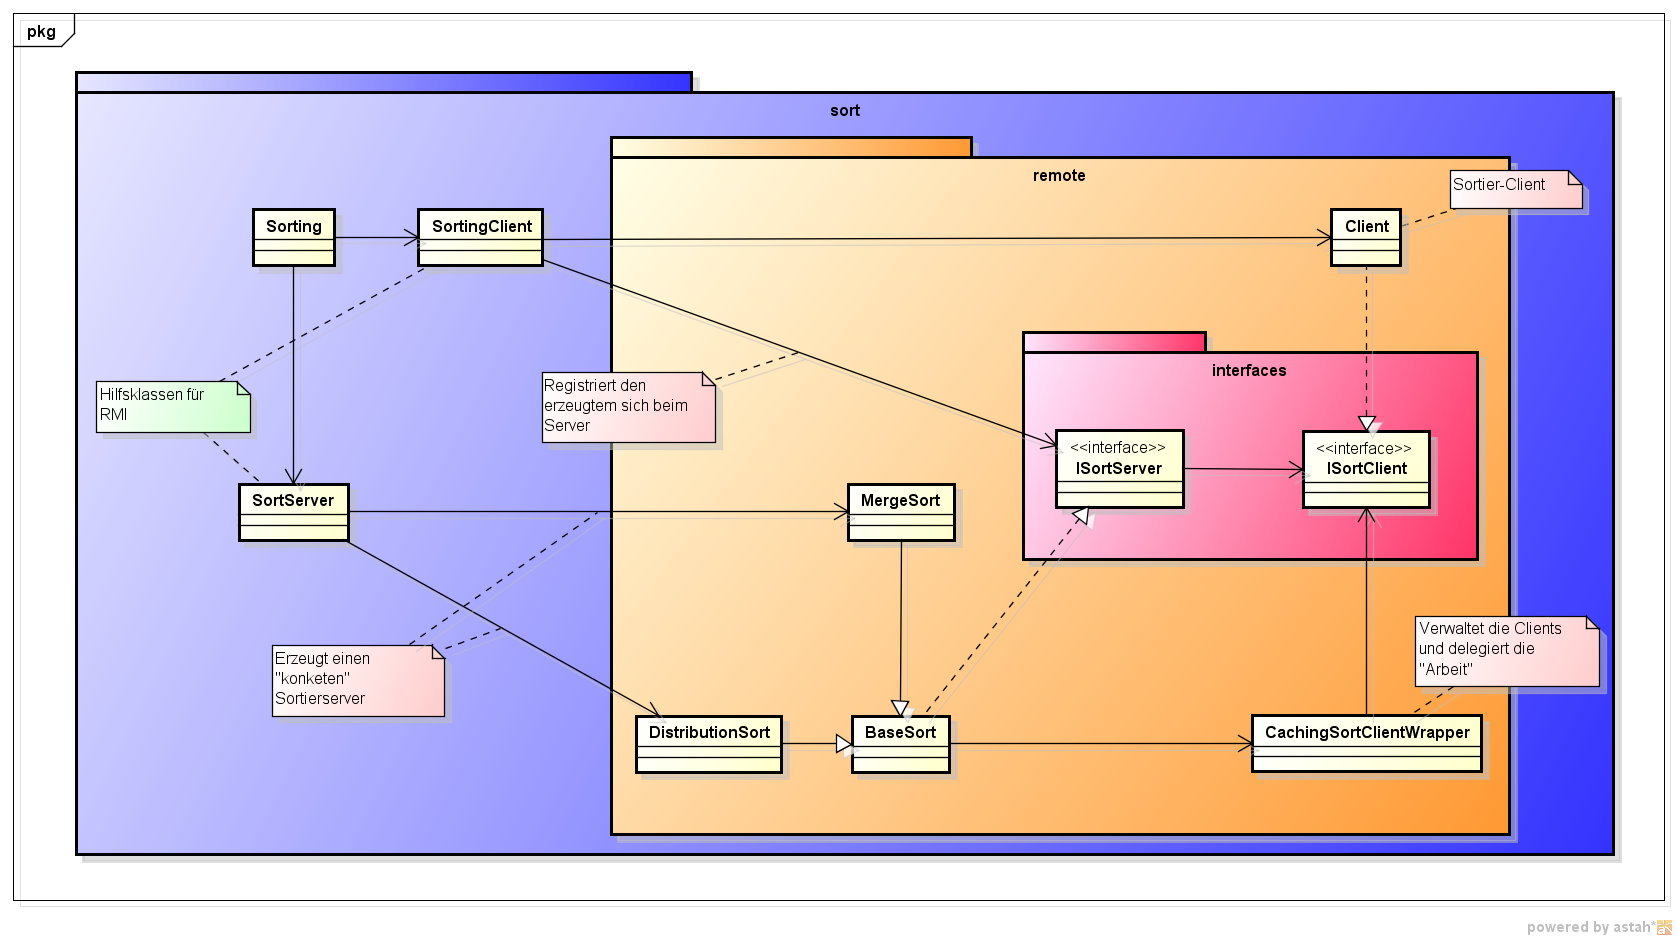
\includegraphics[width=\textwidth]{Klassenstruktur.png}
	\caption{Klassenstruktur: Sortierclient und -server}
\end{figure}
\end{appendix}

\end{document}

